\documentclass[aspectratio=169]{beamer}
\usepackage{caption}        % caption in two lines
\usepackage{subcaption}
\usepackage[utf8]{inputenc} % codificacao de caracteres
\usepackage[T1]{fontenc}    % codificacao de fontes
\usepackage[brazil]{babel}  % idioma
\usepackage{graphicx}       %fundo
\usetheme{default}          % tema
\usecolortheme{orchid}     % cores
\usefonttheme[onlymath]{serif} % fonte modo matematico

\usepackage{subcaption}

\usepackage{listings}
\lstset{%frame=tb,
  language=C,
  aboveskip=3mm,
  belowskip=3mm,
  showstringspaces=false,
  columns=flexible,
  %basicstyle={\small\ttfamily},
  numbers=none,
  %numberstyle=\tiny\color{gray},
  %keywordstyle=\color{blue},
  %commentstyle=\color{dkgreen},
  %stringstyle=\color{mauve},
  breaklines=true,
  breakatwhitespace=true,
  tabsize=3
}

\beamertemplatenavigationsymbolsempty % Desativando os botoes de navegacao

% Tela cheia
\hypersetup{pdfpagemode=FullScreen}

% Titulo
\makeatletter
\newcommand\titlegraphicii[1]{\def\inserttitlegraphicii{#1}}
\titlegraphicii{}
\setbeamertemplate{title page}
{
  \vbox{}
   {\usebeamercolor[fg]{titlegraphic}\inserttitlegraphic\hfill\inserttitlegraphicii\par}
  \begin{centering}
    \begin{beamercolorbox}[sep=2pt,center]{institute}
      \usebeamerfont{institute}\insertinstitute
    \end{beamercolorbox}
    \begin{beamercolorbox}[sep=12pt,center]{title}
      \usebeamerfont{title}\inserttitle\par%
      \ifx\insertsubtitle\@empty%
      \else%
        \vskip0.2em%
        {\usebeamerfont{subtitle}\usebeamercolor[fg]{subtitle}\insertsubtitle\par}%
      \fi%     
    \end{beamercolorbox}%
    \vskip0.2em\par
    \begin{beamercolorbox}[sep=2pt,center]{author}
      \usebeamerfont{author}\insertauthor
    \end{beamercolorbox}
    %\begin{beamercolorbox}[sep=4pt,center]{date}
      %\usebeamerfont{date}\insertdate
    %\end{beamercolorbox}%\vskip0.5em
  \end{centering}
  %\vfill
}
\makeatother
\title{INTEPRETAÇÃO DOS DIALETOS RS274-D E EXTRAÇÃO DOS DADOS 
TEMPORAIS DA USINAGEM EM MÁQUINAS CNC}
%\subtitle{Subtítulo}
\author{\textbf{Francisco Ricardo Taborda Aguiar}}
\institute{UNIVERSIDADE FEDERAL DO PARANÁ \\ 
PROGRAMA DE PÓS GRADUAÇÃOEM ENGENHARIA DE MANUFATURA \\
MESTRADO PROFISSIONAL EM ENGENHARIA DE MANUFATURA} % opcional


\AtBeginSubsection[]
{
  \begin{frame}<beamer>{Assuntos}   
    \tableofcontents[currentsection,currentsubsection]
  \end{frame}
}

% Let's get started
\begin{document}
{%
 \usebackgroundtemplate{
  \centering
  
\includegraphics[width=\paperwidth]{CapaUFPR2.png}
 }
\begin{frame}
  \titlepage
\end{frame}
}
{%
 \usebackgroundtemplate{
  \centering
  
\includegraphics[width=\paperwidth]{FundoUFPR3.png}
 }
\begin{frame}{Assuntos}
  \tableofcontents
  % You might wish to add the option [pausesections]
\end{frame}

% Section and subsections will appear in the presentation overview
% and table of contents.

\section{Introdução}

\subsection{Contexto}

\begin{frame}
  \frametitle{Contexto}

  \begin{itemize}
    \item A usinagem \'e uma atividade relevante na ind\'ustria de 
          manufatura estando presente em diversos tipos de indústria.
    \item Na ind\'ustria metal\'urgica, a transforma\c c\~ao 
          dos materiais met\'alicos ocorre, principalmente, atrav\'es 
          do uso de m\'aquinas CNC.
    \item Conhecer o tempo real de usinagem e relacioná-lo com os demais 
          parâmetros significativos do processo é fundamental para o 
          planejamento da produção e para a definição dos custos das 
          operações.
    \item Obter o tempo real de usinagem corresponde a uma grande 
          dificuldade no processo de fabricação.
    \item As estimativas feitas pelos sistemas CAM podem ser muito 
          inferiores ao tempo real.
  \end{itemize}

\end{frame}


\begin{frame}
  \frametitle{Contexto}
  \begin{itemize}
    \item A comunicação, o compartilhamento e a troca de dados é um fator 
          importante para o processo de digitalização da linha de produção 
          na indústria.
    \item Os Engenheiros e Especialistas demandam um acesso r\'apido 
          e estruturado dos dados coletados ao longo do processo de 
          manufatura.
    \item A digitaliza\c c\~ao do planejamento e o desenvolvimento de um 
          processo de produ\c c\~ao moderno utilizam o conceito de 
          \emph{Gêmeos Digitais} ao inv\'es de prot\'otipos f\'isicos da 
          linha de produ\c c\~ao.
    \item Porém, o processo de constru\c c\~ao de um \emph{Gêmeo Digital} 
          demanda um modelo de informa\c c\~ao padronizado.
    \item A extra\c c\~ao de dados das m\'aquinas demanda o uso 
          de tecnologias espec\'ificas. 
  \end{itemize}  

\end{frame}


\begin{frame}{MT Connect}

  \begin{itemize}

    \item {
      MTConnect \'e um padr\~ao para a troca de dados e informa\c c\~oes 
      que \'e baseado em um dicion\'ario de dados de termos que descrevem 
      informa\c c\~oes associadas com as opera\c c\~oes da fabrica\c c\~ao.
    }

    \item {
      Demanda a implanta\c c\~ao de adaptadores ou de sistemas 
      invasivos para que ocorra a integra\c c\~ao dos dados.      
    }   

  \end{itemize}   

\end{frame}


\begin{frame}{OPC-UA}

  \begin{itemize}

    \item {
      Especifica um modelo de informa\c c\~ao para a representa\c c\~ao 
      de uma m\'aquina-ferramenta, fornecendo condi\c c\~oes para permitir
      a troca de informa\c c\~oes entre uma m\'aquina-ferramenta e softwares
      como MES, SCADA, ERP, ou sistemas de an\'alise de dados.
    }

    \item {
      Disponível somente em equipamentos mais modernos e fornecedores 
      específicos.
    }

  \end{itemize}   

\end{frame}




\begin{frame}{Interoperabilidade}

  \begin{itemize}
    
    \item {
      A diversidade dos dialetos resultaram na falta de interoperabilidade
      entre as máquinas \emph{CN}.
    }

    \item {
      A mesma pe\c ca necessita de programas diferentes para ser usinada 
      em m\'aquinas de fornecedores diferentes.
    }

    \item {
      A integração entre os sistemas \emph{CN} com outros sistemas 
      (\emph{CAPP}, por exemplo) são comprometidos pela falta de 
      interoperabilidade.
    }

  \end{itemize}   

\end{frame}

\subsection{Objetivos}

\begin{frame}{Objetivo Geral}
  \begin{itemize}
    \item { 
      Desenvolver uma metodologia para interpretar os diferentes dialetos 
      do formato \emph{RS274-D} e gerar um modelo granular de dados, 
      no qual cada movimento da m\'aquina \'e registrado com uma marcação 
      de tempo.
    }
  \end{itemize}
\end{frame}

\begin{frame}{Objetivos Específicos}
  \begin{itemize}
    \item Projetar uma estrutura de dados que contemple dois objetivos:
    \begin{itemize}
        \item Possibilitar o registro temporal dos eventos decorrentes do 
              processamento do programa de controle numérico.
        \item Formar uma camada abstrata de dados que possa ser utilizada
              para tratar das questões da interoperabilidade entre os 
              dialetos.
    \end{itemize}
    \item Representar, por meio de diagramas abstratos, a metodologia proposta na dissertação.
    \item Implementar um estudo de caso a partir de um dialeto específico.
\end{itemize}
\end{frame}


\section{Revisão Bibliográfica}


\subsection{Gêmeos Digitais}

\begin{frame}{Gêmeos Digitais}

  TODO

\end{frame}  


\subsection{Padrão RS274-D}

\begin{frame}{Origem}
  \begin{itemize}
  \item {
    Nos anos sessenta, a Electronic Industry Association (EIA) desenvolveu um 
    padrão conhecido como RS274-D para programar máquinas CNC.
  }
  \item {
    A mídia de armazenamento comum era baseada nos cartões perfurados.
  }
  \item {
    O hardware era restrito.
  }
  \item {
    Os caracteres eram representados no padrão ASCII (American Standard Code for Information Interchange).
  }
  \item {
    Em 1982 o padrão foi adotado pela ISO sendo chamado de ISO 6983.
  }
  \end{itemize}
\end{frame}


\begin{frame}{Objetivos}
  \begin{itemize}
  \item {
    Promover a uniformidade de técnicas de programação.
  }
  \item {
    Favorecer a intercambiabilidade de programas entre diferentes máquinas de controle numérico.
  }
  \item {
    Máquinas simples possam ser programadas com um formato simples de programa,
    o qual possa se extensível para máquinas mais complexas.
  }
  \end{itemize}
\end{frame}


\begin{frame}{Arquitetura}
  \begin{itemize}
  \item {
    Os programas são organizados em linhas de código, também chamados de blocos.
  }
  \item {
    Um bloco consiste de um número de linha opcional no início do bloco, seguido por um 
    ou mais comandos.
  }
  \item {
    Um comando (ou palavra) corresponde a uma letra sucedida por um sinal algébrico, se aplicável, 
    seguido por um número ou por uma expressão que pode ser avaliada para um número.
  }
  \end{itemize}
\end{frame}


\begin{frame}{Exemplos de alguns comandos RS274/NGC}

  \scriptsize{Fonte: KRAMER, T.; PROCTOR, F. 
    The NIST RS274/VGER Interpreter. US Department of
    Commerce, National Institute of Standards e Technology, set. 1998.}

  \begin{table}[H]
    \centering
    \begin{tabular}{p{7cm}|p{5cm}}
    
      \hline
      \bfseries{\scriptsize{Comandos}} & \bfseries{\scriptsize{Prop\'osito}} \\
  
      \hline
      \scriptsize{G0, G1, G2, G3, G38, G80, G81, G82, G83, G84, G85, G86, G87, G88, G89} 
      & \scriptsize{Movimento} \\
  
      \hline
      \scriptsize{G17, G18, G19} 
      & \scriptsize{Sele\c c\~ao do plano} \\
  
      \hline
      \scriptsize{G90, G91}
      & \scriptsize{Modo das dist\^ancias} \\
  
      \hline
      \scriptsize{G93, G94}
      & \scriptsize{Modo da velocidade de corte} \\
  
      \hline
      \scriptsize{G20, G21}
      & \scriptsize{Unidade} \\
  
      \hline
      \scriptsize{G40, G41, G42}
      & \scriptsize{Compensa\c c\~ao do di\^ametro de corte} \\
  
      \hline
      \scriptsize{G43, G49}
      & \scriptsize{Dist\^ancia da ferramenta} \\
  
      \hline
      \scriptsize{G98, G99}
      & \scriptsize{Modo de retorno em ciclos fixos} \\
  
      \hline
      \scriptsize{G54, G55, G56, G57, G58, G59, G59.1, G59.2, G59.3}
      & \scriptsize{Sele\c c\~ao do sistema de coordenadas} \\
  
      \hline
      \scriptsize{M0, M1, M2, M30, M60}
      & \scriptsize{Parada} \\
  
      \hline
      \scriptsize{M6}
      & \scriptsize{Troca de ferramenta} \\
  
      \hline
      \scriptsize{M3, M4, M5}
      & \scriptsize{Sentido do giro do eixo} \\
  
      \hline
      \scriptsize{M7, M8, M9}
      & \scriptsize{Refrigera\c c\~ao} \\
  
      \hline
      \scriptsize{M48, M49}
      & \scriptsize{Interruptor do avan\c co e do corte} \\

      \hline
  
    \end{tabular}
  \end{table}

\end{frame}


\subsection{Dialetos}

\begin{frame}{Dialetos}
  \begin{itemize}
  \item {
    Os padrões são apenas nominais hoje em dia.     
  }
  \item {   
    A tecnologia dos sistemas CNC avançou muito desde que as normas 
    foram publicadas.
  }
  \item {
    Os fabricantes de máquinas têm estendido o padrão \emph{RS274-D}, 
    criando novos comandos ou adaptando comandos existentes, levando 
    ao surgimento de vários dialetos. 
  }
  \end{itemize}
\end{frame}


\begin{frame}{Exemplos}
  \begin{itemize}
    \item {
      Fonte: Adaptado de ZHANG, X.; NASSEHI, A.; NEWMAN, S. T. A meta-model of computer numerical
      controlled part programming languages. Proceedings of the Institution of
      Mechanical Engineers, Part B: Journal of Engineering Manufacture, Sage
      Publications Sage UK: London, England, v. 229, n. 7, p. 1243-1257, 2015.
      \begin{table}[H]
        \centering    
        {\begin{tabular}{p{4.3cm}|p{2.6cm}|p{2.4cm}}
          \hline
          \bfseries{\footnotesize{Comando}} & 
          \bfseries{\footnotesize{Fanuc}} & 
          \bfseries{\footnotesize{Siemens}} \\
      
          \hline
          \footnotesize{Interpolação Linear} & 
          \footnotesize{G01 X...Y...} & 
          \footnotesize{G1 X...Y...} \\
      
          \hline
          \footnotesize{Interpolação Circular (Horário)} & 
          \footnotesize{G02 X...Y...I...J...} & 
          \footnotesize{G2 X...Y...I...J...} \\
      
          \hline
          \footnotesize{Ciclo Fixo de Furação} & 
          \footnotesize{G83...} & 
          \footnotesize{CYCLE G83...} \\
      
          \hline
          \footnotesize{Definição da Unidade} & 
          \footnotesize{G20 ou G21 } & 
          \footnotesize{G70 ou G71} \\

          \hline

        \end{tabular}}
      \end{table}
    }    
  \end{itemize}
\end{frame}


\subsection{Padrão STEP-NC}

\begin{frame}{Origem}
  \begin{itemize}
  \item {
    Esforço realizado pelo Comitê Técnico da ISO 184 (Sistemas de Automação Industrial e
    Integração) para enfrentar o problema com interoperabilidade e integração.
  }
  \item {
    Formalizado na norma ISO 10303 (Padrão Internacional para a representação e troca de dados do produto).
  }  
  \item {
    O padrão ISO 14649 (STEP-NC) define um modelo para a transferência de dados entre sistemas CAD/CAM.
  }
  \item {
    Correspode a um modelo mais completo de informações para descrever processos de usinagem.
    \begin{itemize}
      \item A geometria da peça.
      \item Os features da usinagem.
      \item A sequência de operações.
      \item Os parâmetros de processo.
      \item As especificações de ferramentas.
    \end{itemize}
  }
  \end{itemize}
\end{frame}

%\subsection{Objetivos}

\begin{frame}{Objetivos}
  \begin{itemize}
    \item {
      Substituir o padrão RS274-D / ISO 6983.
    }
    \item{
      A criação de um padrão internacional que seja único capaz de cobrir todos os aspectos 
      da transferência de dados entre sistemas CAD/CAM.
    }
    \item {
      A padronização de um mecanismo para descrever os dados do produto, ao longo do ciclo de 
      vida do produto.
    }
    \item {
      Formato neutro para a troca de dados.
    }
    \item {
      Fazer a separação entre a descrição do produto e a sua implementação, 
      de forma independente de sistemas particulares.
    }
    \item {
      Capaz de fornecer as bases para o compartilhamento de bancos de dados de produtos.
    }
  \end{itemize}
\end{frame}


%\subsection{Exemplo}

\begin{frame}{Exemplo}

  Adaptado de POBOZNIAK, J.; SOBIESKI, S. Extension of STEP-NC data structure to represent
  manufacturing process structure in CAPP system. Procedia Manufacturing, Elsevier,
  v. 11, p. 1692-1699, 2017.

  \begin{figure}[H]
    \centering
    \begin{subfigure}[b]{0.46\textwidth}
        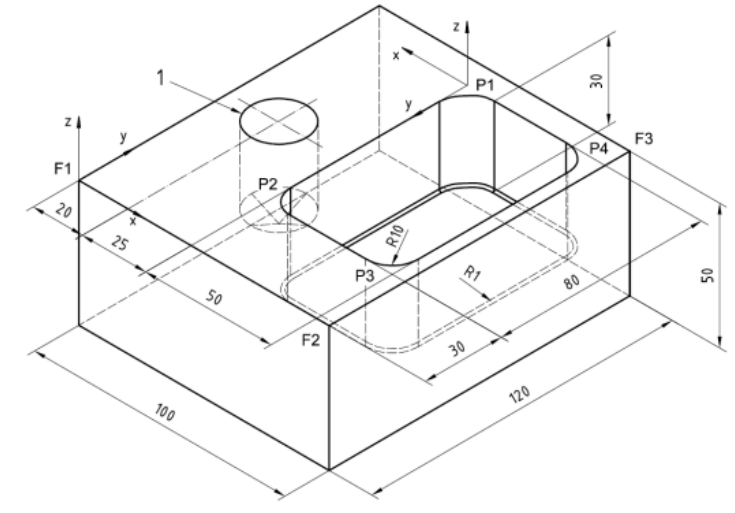
\includegraphics[width=\textwidth]{part1.png}
    \end{subfigure}
    \qquad
    \begin{subfigure}[b]{0.46\textwidth}
        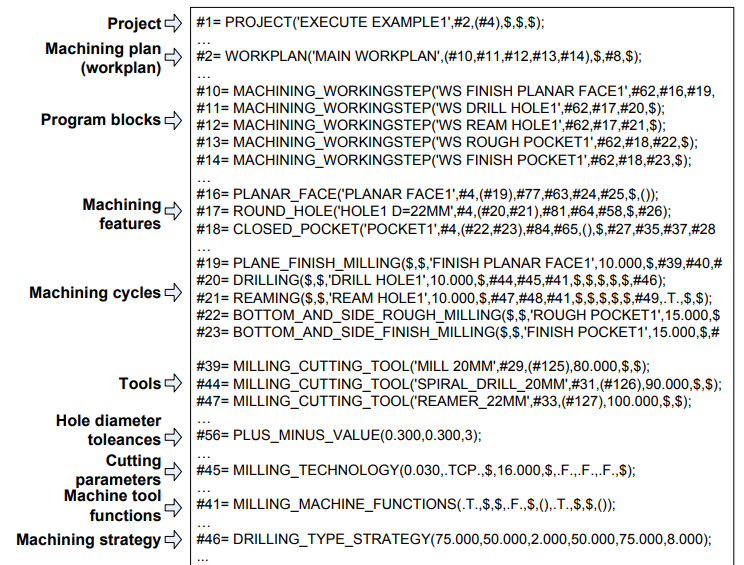
\includegraphics[width=\textwidth]{step-nc-sample-1.png}
    \end{subfigure}
\end{figure}

\end{frame}

%\subsection{Problema}

\begin{frame}{Considerações}

  \begin{itemize}
    \item {
      Apesar do interesse em torno do formato STEP-NC e da inovação tecnológica
      que vem acontecendo nos equipamentos de CNC, o formato RS274-D ainda é dominante.
    }
    \item {
      Os processos de usinagem ainda dependem de máquinas antigas controladas
      por sistemas NC proprietários que são dialetos das normas RS274-D ou ISO 6983.
    }
  \end{itemize}   

\end{frame}


\subsection{Funções Canônicas de Usinagem}

\begin{frame}{Funções Canônicas de Usinagem}
  \begin{itemize}
    \item{
      A Intelligente Systems Division (ISD) do National Institute of 
      Standards and Technology (NIST) trabalhou no projeto 
      Enhanced Machine Controller (EMC), de forma colaborativa com 
      outros parceiros.
    }
    \item {
      O objetivo do projeto foi construir um padrão de interface de 
      programação de aplicações (API) para controladores de máquinas 
      com arquitetura aberta. 
      Além disto, demonstrar as implementações da arquitetura do 
      Next Generation Controller (NGC).
    }
  \end{itemize}
\end{frame}


\begin{frame}{Objetivos}
  \begin{itemize}    
    \item {
      As Funções Canônicas de Usinagem (do Inglês, CMF, Canonical 
      Machining Functions) foram projetadas com três objetivos em mente.
      \begin{itemize}        
        \item {
          Todas as funcionalidades dos centros de usinagem de 3 a 6 
          eixos devem ser cobertas pelos comandos.
        }
        \item {
          Os comandos canônicos de movimento devem ser portáveis para 
          serem reconhecidos em placas de controle comerciais 
          disponíveis no mercado.         
        }
        \item {
          Deve ser possível interpretar comandos RS274-D em chamadas de 
          Funções Canônicas de Usinagem.
        }
      \end{itemize}
    }
    \item {
      O projeto EMC e outros projetos abertos de pesquisa em máquinas 
      CNC utilizam CMFs.
    }
    \item {
      As Funções Canônicas de Usinagem consistem em comandos atômicos.
      Os comandos RS274-D podem ser decompostos em várias chamadas de CMFs.
    }
  \end{itemize}
\end{frame}


\begin{frame}{Exemplos de comandos}
  \begin{table}[H]
    \centering
    \begin{tabular}{p{7cm}|p{5cm}}

      \hline
      \bfseries{\scriptsize{Comandos}} & \bfseries{\scriptsize{Prop\'osito}} \\

      \hline  
      \scriptsize{SET\_TRAVERSE\_RATE (double \emph{rate})} 
      & \scriptsize{Define o valor superior da velocidade do movimento de aproxima\c c\~ao 
      que ser\'a utilizado durante os movimentos r\'apidos que ocorrem, normalmente, quando 
      o equipamento n\~ao est\'a fazendo opera\c c\~oes de corte.} \\

      \hline      
      \scriptsize{STRAIGHT\_TRAVERSE (double \emph{x}, double \emph{y}, double \emph{z}, 
      double \emph{a}, double \emph{b}, double \emph{c})} 
      & \scriptsize{Faz um movimento de posicionamento linear a partir da posi\c c\~ao 
      atual at\'e o ponto definido por \emph{x}, \emph{y}, \emph{z}, \emph{a}, \emph{b} e \emph{c}.
      \'E esperado que n\~ao ocorra opera\c c\~ao de corte durante o movimento de travessia.} \\

      \hline  
      \scriptsize{SET\_FEED\_RATE (double \emph{rate})}
      & \scriptsize{Define a velocidade de avan\c co.} \\

      \hline  
      \scriptsize{STRAIGHT\_FEED (double \emph{x}, double \emph{y}, double \emph{z}, 
      double \emph{a}, double \emph{b}, double \emph{c})} 
      & \scriptsize{Move em linha reta, na velocidade de avan\c co previamente definida, 
      a partir da posi\c c\~ao atual at\'e a 
      posi\c c\~ao dada por \emph{x}, \emph{y} e \emph{z}.} \\

      \hline  
      \scriptsize{SET\_SPINDLE\_SPEED (double \emph{speed})} 
      & \scriptsize{Define a velocidade de rotação} \\

      \hline

    \end{tabular}
  \end{table}
\end{frame}


\begin{frame}{Considerações}

  \begin{itemize}
    \item Assim como ocorre com o \emph{STEP-NC}, o formato baseado nas 
          Funções Canônicas de Usinagem não tem sido amplamente adotado 
          entre os controladores de CNC comerciais.
    \item A atomicidade das Funções Canônicas de Usinagem representa uma 
          característica interessante para o registro temporal de cada 
          evento que ocorre na máquina-ferramenta durante o processamento 
          do programa.
    \item A simplicidade da sintaxe e a padronização das chamadas de 
          funções são pontos positivos para a construção de uma camada 
          de abstração a partir das Funções Canônicas de Usinagem.
    \emph{CN}.

  \end{itemize}

\end{frame}




\begin{frame}{Pós-processadores}

  \begin{itemize}

    \item {
      São softwares ou sub-rotinas 
      que convertem um arquivo gerado em um sistema \emph{CAM} 
      em um programa que possa ser identificado em um 
      determinado sistema \emph{CN}.
    }
    
    \item {
      Porém, há um número elevado tanto de sistemas
      \emph{CAM} quanto de fornecedores de máquinas \emph{CNC}, 
      o que faz com que a demanda por Pós-Processadores
      tenha que ser muito alta.
    }

  \end{itemize}   

\end{frame}





\subsection{Transpilação}

\begin{frame}
  \frametitle{Transpilação}

  TODO
  Análise Léxica
  Expressões Regulares
  Análise Sintática
  Gramática Livre de contexto
  Algoritmo LR
  

\end{frame}




\section{Metodologia}

\begin{frame}{Módulos}
  \begin{enumerate}
    \item {
      \emph{Transpiler}: 
      \begin{itemize}
        \item Interpretar o formato \emph{RS274-D};
        \item Adaptável aos diversos dialetos RS274-D;
        \item Elevar o nível de abstração dos dados para um formato 
              neutro (independente de tecnologias proprietárias).
        \item Processar o formato neutro e gerar as marcações de tempo.
      \end{itemize}
    }

    \item {
      \emph{Persistence}:
      \begin{itemize}
        \item Armazenar e restaurar os dados do tipo \emph{Payload}.
        \item Foi definida uma arquitetura orientada a documentos 
              (\emph{NoSQL}) para o banco de dados, pois o sistema 
              proposto não apresenta uma natureza relacional.
      \end{itemize}
    }

    \item {
      \emph{Output}
      \begin{itemize}
        \item Interpretar a lista de objetos \emph{Payload} 
              e gerar dois tipos de saída:
        \begin{itemize}
              \item Um arquivo com os dados temporais da usinagem. 
                    Em formato \emph{CSV}, para facilitar a importação 
                    do arquivo em softwares de análise de dados.
              \item Um arquivo em formato de Funções Canônicas de Usinagem.
        \end{itemize}
      \end{itemize}
    }

  \end{enumerate}
\end{frame}


\begin{frame}{Visão Geral}

  \begin{figure}[H]
    \centering
    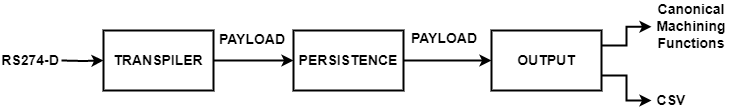
\includegraphics[width=\textwidth]{images/idef0-main.png}
  \end{figure}

\end{frame}


\begin{frame}{Diagrama de Classes Conceitual}

  \begin{figure}[H]
    \centering
    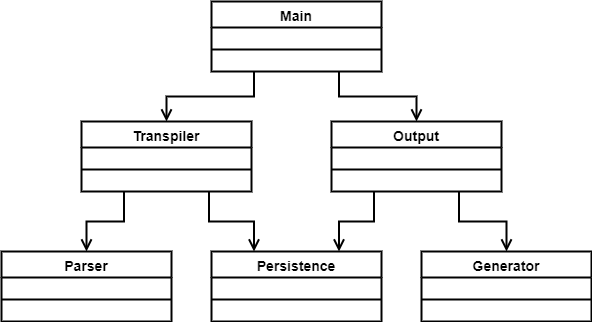
\includegraphics[width=90mm]{images/class-main.png}
  \end{figure}

\end{frame}


\begin{frame}{Transpiler}
  \begin{itemize}
    \item Abordagem baseada em um fluxo de duas etapas:
    \begin{enumerate}
      \item Análise Léxica (ou \emph{Scanning}).
      \item Análise Sintática (ou \emph{Parsing}).
    \end{enumerate}
  \end{itemize}
\end{frame}


\begin{frame}{Etapa 1}
  \begin{itemize}
    \item A primeira etapa (\emph{Scanner}) l\^e a entrada e traduz as 
          cadeias de caracteres em símbolos (tokens). 
    \item Uma ferramenta chamada \emph{Flex} foi utilizada para esta 
          implementa\c c\~ao.
    \item Os tokens são identificados a partir de Expressões Regulares.
  \end{itemize}
\end{frame}


\begin{frame}[fragile]
  \frametitle{Exemplo de Expressões Regulares}
  \begin{example}
      "G1X10.Y3.5Z-1.F505"
      \begin{lstlisting}
        GCODE = 'G'        
        INT = '[0-9]+'
        X = '[Xx]'
        Y = '[Yy]'
        Z = '[Zz]'
        F = 'F'
        FLOAT = '[+-]?[0-9]+[.]?[0-9]*'
      \end{lstlisting}
    \end{example}
  \end{frame}


  \begin{frame}
    \frametitle{Detalhamento da Expressão Regular \emph{FLOAT}}
    \begin{itemize}
      \item \emph{FLOAT} = \emph{'[+-]?[0-9]+[.]?[0-9]*'}
        \begin{itemize}
          \item \emph{[-+]}: um caractere \emph{+} ou \emph{-}.
          \item \emph{?}: o caractere anterior (no caso, \emph{+} ou \emph{-}) deve aparecer 0 ou 1 vez.
          \item \emph{[0-9]}: um dígito (de 0 até 9).
          \item \emph{+}: o caractere anterior (no caso, um dígito) deve aparecer 1 ou mais vezes.
          \item \emph{[.]}: um ponto final (\emph{.}).
          \item \emph{?}: o caractere anterior (no caso, um ponto final) deve aparecer 0 ou 1 vez.
          \item \emph{[0-9]}: um dígito (de 0 até 9).
          \item \emph{*}: o caractere anterior (no caso, um dígito) deve aparecer 0 ou muitas vezes.
      \end{itemize}
    \end{itemize}
\end{frame}


\begin{frame}{Etapa 2}
  \begin{itemize}
    \item A segunda etapa (\emph{Parser}) agrupa os símbolos em unidades 
          sint\'aticas (no caso, blocos de comandos).
    \item Utiliza uma Gramática Livre de Contexto (Context-Free Grammar).
    \item Consiste em um conjunto de regras gramaticais que descrevem a 
          sintaxe de uma determinada linguagem (no caso, um dialeto RS274-D).
    \item Extensível para os diversos dialetos.
    \item A sintaxe do dialeto é descrita através da notação Backus-Naur 
          Form (BNF).
    \begin{itemize}
      \item Linguagens de programação, formatos de documentos e 
            protocolos de comunicação.
    \end{itemize}
    \item O processamento é feito por um algoritmo \emph{LR}, baseado no método 
          \emph{Shift-Reduce}, amplamente utilizado para o processamento 
          de linguagens de computação.
  \end{itemize}
\end{frame}


\begin{frame}[fragile]
  \frametitle{Exemplo de Especificação BNF}
  \begin{example}
   "G1X10.Y3.5Z-1.F505"
    \begin{lstlisting}
      machining : GCODE "1" position F INT

      position : X FLOAT
               | Y FLOAT
               | Z FLOAT
               | X FLOAT Y FLOAT
               | X FLOAT Z FLOAT
               | Y FLOAT Z FLOAT
               | X FLOAT Y FLOAT Z FLOAT
    \end{lstlisting}
  \end{example}  
\end{frame}


\section{Estudo de Caso}

\begin{frame}
  \frametitle{Estudo de Caso}
  \framesubtitle{Implementação}

  \begin{itemize}
    \item Implementação do \emph{Transpiler} em \emph{C} e \emph{C++}.
    \item Ambiente de desenvolvimento em \emph{Docker}, 
          imagem \emph{Debian Bullseye}.
    \item \emph{IDE Microsoft Visual Studio Code}.
    \item Compilador \emph{GCC}.
    \item O foco da implementação foi testar o processo de transpilação 
          e avaliar os resultados obtidos com esse processo.
  \end{itemize}

  \end{frame}


\begin{frame}
  \frametitle{Estudo de Caso}
  \framesubtitle{Protótipo}

  \begin{itemize}
    \item Controlador de CNC modelo \emph{Mach-9}, fornecedor 
          \emph{Romi - Brasil}, disponível em um centro de usinagem de
           três eixos modelo \emph{Discovery 4022}.
    \item O controlador \emph{Mach-9} utiliza um dialeto do padrão 
          \emph{RS274-D}.
    \item O programa \emph{CN} foi gerado no software \emph{CAM} 
          \emph{Edgecam 2019 R2} (\emph{Hexagon} - Suécia), que tem um 
          pós-processador para o dialeto \emph{Mach-9}.
  \end{itemize}

\end{frame}


\begin{frame}
  \frametitle{Estudo de Caso}
  \framesubtitle{Análise Léxica}
  \begin{itemize}
    \item A implementação do \emph{Scanner} utilizou o software 
          \emph{Flex} e Expressões Regulares para extrair os símbolos.
    \item Exemplos:
      \begin{itemize}
        \item Select tool: \emph{[T][0]?[1-9]+}
        \item Change tool: \emph{[M][0]?[6]}
        \item Set spindle speed: \emph{[S][0-9]+}
        \item Spindle clockwise: \emph{[M][0]?[3]}
      \end{itemize}  
  \end{itemize}

\end{frame}


\begin{frame}[fragile]
  \frametitle{Estudo de Caso}
  \framesubtitle{Análise Sintática}
  \begin{itemize}
    \item A implementação do \emph{Parser} utilizou o software 
          \emph{Bison}.
    \item Foi definida a Gramática Livre de Contexto de acordo com o 
          dialeto \emph{Mach-9} e um algoritmo \emph{LR}
          para processar os símbolos.
    \item Exemplos da Gramática Livre de Contextos:
      \begin{lstlisting}
        spindle : SET_SPINDLE_SPEED
        | SPINDLE_CLOCKWISE
        | SPINDLE_COUNTER_CLOCKWISE
        | SET_SPINDLE_SPEED SPINDLE_CLOCKWISE
        | SET_SPINDLE_SPEED SPINDLE_COUNTER_CLOCKWISE
        | STOP_SPINDLE_TURNING
      
        tool : SELECT_TOOL
        | SELECT_TOOL CHANGE_TOOL    
    \end{lstlisting}
  \end{itemize}

\end{frame}  


\begin{frame}[fragile]
  \frametitle{Estudo de Caso}
  \framesubtitle{Trecho do programa \emph{CN}}

  A tabela abaixo apresenta um trecho do programa \emph{CN}.

  \vspace{3mm}

  \begin{tabular}{l|l}
    \hline
    \scriptsize{\bfseries{NÚMERO DA LINHA}} & 
    \scriptsize{\bfseries{G-CODE}} \\
    \hline

    \scriptsize{1} & \scriptsize{T3M6} \\    
    \hline

    \scriptsize{2} & \scriptsize{O3S1857M3} \\
    \hline

    \scriptsize{3} & \scriptsize{G0X-15.Y-65.Z3.} \\
    \hline
      
    \scriptsize{4} & \scriptsize{X-15.Y-65.Z5.} \\
    \hline

    \scriptsize{5} & \scriptsize{G81Z-8.R3.F186} \\
    \hline

    \scriptsize{6} & \scriptsize{G25X30.Y130.I2J2} \\
    \hline

    \scriptsize{7} & \scriptsize{G80} \\
    \hline

    \scriptsize{8} & \scriptsize{M5} \\
    \hline
      
  \end{tabular}

\end{frame}  


\begin{frame}[fragile]
  \frametitle{Estudo de Caso}
  \framesubtitle{Resultados e Discussões}

  As tabelas a seguir apresentam os campos mais relevantes que são 
  resultado da transpilação dos blocos 5, 6 e 7 do programa \emph{CN}.

  \vspace{3mm}

  \begin{tabular}{|l|l|l|l|l|l|l|l|l|l|}

    \hline

    \tiny{\bfseries{function\_name}} & 
    \tiny{\bfseries{x1}} & 
    \tiny{\bfseries{y1}} & 
    \tiny{\bfseries{z1}} & 
    \tiny{\bfseries{feed}} & 
    \tiny{\bfseries{speed}} & 
    \tiny{\bfseries{tool}} & 
    \tiny{\bfseries{time}} & 
    \tiny{\bfseries{timestamp}} \\
    \hline

    \tiny{\bfseries{SELECT\_TOOL}} & 
    \tiny{\bfseries{-9.0}} & 
    \tiny{\bfseries{15.59}} & 
    \tiny{\bfseries{3.0}} & 
    \tiny{\bfseries{0}} & 
    \tiny{\bfseries{0}} & 
    \tiny{\bfseries{3}} & 
    \tiny{\bfseries{7}} & 
    \tiny{\bfseries{91.191}} \\    
    \hline

    \tiny{\bfseries{CHANGE\_TOOL}} & 
    \tiny{\bfseries{-9.0}} & 
    \tiny{\bfseries{15.59}} & 
    \tiny{\bfseries{3.0}} & 
    \tiny{\bfseries{0}} & 
    \tiny{\bfseries{0}} & 
    \tiny{\bfseries{3}} & 
    \tiny{\bfseries{0}} & 
    \tiny{\bfseries{91.191}} \\
    \hline

    \tiny{\bfseries{SET\_SPINDLE\_SPEED}} & 
    \tiny{\bfseries{-9.0}} & 
    \tiny{\bfseries{15.59}} & 
    \tiny{\bfseries{3.0}} & 
    \tiny{\bfseries{0}} & 
    \tiny{\bfseries{1857}} & 
    \tiny{\bfseries{3}} & 
    \tiny{\bfseries{0}} & 
    \tiny{\bfseries{91.191}} \\
    \hline

    \tiny{\bfseries{START\_SPINDLE\_CLOCKWISE}} & 
    \tiny{\bfseries{-9.0}} & 
    \tiny{\bfseries{15.59}} & 
    \tiny{\bfseries{3.0}} & 
    \tiny{\bfseries{0}} & 
    \tiny{\bfseries{1857}} & 
    \tiny{\bfseries{3}} & 
    \tiny{\bfseries{2}} & 
    \tiny{\bfseries{93.191}} \\
    \hline    

    \tiny{\bfseries{STRAIGHT\_TRAVERSE}} & 
    \tiny{\bfseries{-15.0}} & 
    \tiny{\bfseries{-65.0}} & 
    \tiny{\bfseries{3.0}} & 
    \tiny{\bfseries{15000}} & 
    \tiny{\bfseries{1857}} & 
    \tiny{\bfseries{3}} & 
    \tiny{\bfseries{0.323}} & 
    \tiny{\bfseries{93.515}} \\
    \hline

    \tiny{\bfseries{STRAIGHT\_TRAVERSE}} & 
    \tiny{\bfseries{-15.0}} & 
    \tiny{\bfseries{-65.0}} & 
    \tiny{\bfseries{5.0}} & 
    \tiny{\bfseries{15000}} & 
    \tiny{\bfseries{1857}} & 
    \tiny{\bfseries{3}} & 
    \tiny{\bfseries{0.008}} & 
    \tiny{\bfseries{93.523}} \\
    \hline

    \tiny{\bfseries{STRAIGHT\_TRAVERSE}} & 
    \tiny{\bfseries{-15.0}} & 
    \tiny{\bfseries{-65.0}} & 
    \tiny{\bfseries{3.0}} & 
    \tiny{\bfseries{15000}} & 
    \tiny{\bfseries{1857}} & 
    \tiny{\bfseries{3}} & 
    \tiny{\bfseries{0.008}} & 
    \tiny{\bfseries{93.531}} \\
    \hline

    \tiny{\bfseries{SET\_FEED\_RATE}} & 
    \tiny{\bfseries{-15.0}} & 
    \tiny{\bfseries{-65.0}} & 
    \tiny{\bfseries{3.0}} & 
    \tiny{\bfseries{186}} & 
    \tiny{\bfseries{1857}} & 
    \tiny{\bfseries{3}} & 
    \tiny{\bfseries{0}} & 
    \tiny{\bfseries{93.531}} \\
    \hline

    \tiny{\bfseries{STRAIGHT\_FEED}} & 
    \tiny{\bfseries{-15.0}} & 
    \tiny{\bfseries{-65.0}} & 
    \tiny{\bfseries{-8.0}} & 
    \tiny{\bfseries{186}} & 
    \tiny{\bfseries{1857}} & 
    \tiny{\bfseries{3}} & 
    \tiny{\bfseries{3.548}} & 
    \tiny{\bfseries{97.079}} \\
    \hline    

    \tiny{\bfseries{STRAIGHT\_TRAVERSE}} & 
    \tiny{\bfseries{-15.0}} & 
    \tiny{\bfseries{-65.0}} & 
    \tiny{\bfseries{3.0}} & 
    \tiny{\bfseries{15000}} & 
    \tiny{\bfseries{1857}} & 
    \tiny{\bfseries{3}} & 
    \tiny{\bfseries{0.044}} & 
    \tiny{\bfseries{97.123}} \\
    \hline    

    \tiny{\bfseries{STRAIGHT\_TRAVERSE}} & 
    \tiny{\bfseries{15.0}} & 
    \tiny{\bfseries{-65.0}} & 
    \tiny{\bfseries{3.0}} & 
    \tiny{\bfseries{15000}} & 
    \tiny{\bfseries{1857}} & 
    \tiny{\bfseries{3}} & 
    \tiny{\bfseries{0.12}} & 
    \tiny{\bfseries{97.243}} \\
    \hline

  \end{tabular}

\end{frame}  


\begin{frame}[fragile]
  \frametitle{Estudo de Caso}
  \framesubtitle{Resultados e Discussões}

    \begin{tabular}{|l|l|l|l|l|l|l|l|l|l|}

      \hline

      \tiny{\bfseries{function\_name}} & 
      \tiny{\bfseries{x1}} & 
      \tiny{\bfseries{y1}} & 
      \tiny{\bfseries{z1}} & 
      \tiny{\bfseries{feed}} & 
      \tiny{\bfseries{speed}} & 
      \tiny{\bfseries{tool}} & 
      \tiny{\bfseries{time}} & 
      \tiny{\bfseries{timestamp}} \\
      \hline
    

      \tiny{\bfseries{SET\_FEED\_RATE}} & 
      \tiny{\bfseries{15.0}} & 
      \tiny{\bfseries{-65.0}} & 
      \tiny{\bfseries{3.0}} & 
      \tiny{\bfseries{186}} & 
      \tiny{\bfseries{1857}} & 
      \tiny{\bfseries{3}} & 
      \tiny{\bfseries{0}} & 
      \tiny{\bfseries{97.243}} \\
      \hline

      \tiny{\bfseries{STRAIGHT\_FEED}} & 
      \tiny{\bfseries{15.0}} & 
      \tiny{\bfseries{-65.0}} & 
      \tiny{\bfseries{-8.0}} & 
      \tiny{\bfseries{186}} & 
      \tiny{\bfseries{1857}} & 
      \tiny{\bfseries{3}} & 
      \tiny{\bfseries{3.548}} & 
      \tiny{\bfseries{100.791}} \\
      \hline

      \tiny{\bfseries{STRAIGHT\_TRAVERSE}} & 
      \tiny{\bfseries{15.0}} & 
      \tiny{\bfseries{-65.0}} & 
      \tiny{\bfseries{3.0}} & 
      \tiny{\bfseries{15000}} & 
      \tiny{\bfseries{1857}} & 
      \tiny{\bfseries{3}} & 
      \tiny{\bfseries{0.044}} & 
      \tiny{\bfseries{100.835}} \\
      \hline

      \tiny{\bfseries{STRAIGHT\_TRAVERSE}} & 
      \tiny{\bfseries{15.0}} & 
      \tiny{\bfseries{65.0}} & 
      \tiny{\bfseries{3.0}} & 
      \tiny{\bfseries{15000}} & 
      \tiny{\bfseries{1857}} & 
      \tiny{\bfseries{3}} & 
      \tiny{\bfseries{0.52}} & 
      \tiny{\bfseries{101.355}} \\
      \hline    

      \tiny{\bfseries{SET\_FEED\_RATE}} & 
      \tiny{\bfseries{15.0}} & 
      \tiny{\bfseries{65.0}} & 
      \tiny{\bfseries{3.0}} & 
      \tiny{\bfseries{186}} & 
      \tiny{\bfseries{1857}} & 
      \tiny{\bfseries{3}} & 
      \tiny{\bfseries{0}} & 
      \tiny{\bfseries{101.355}} \\
      \hline

      \tiny{\bfseries{STRAIGHT\_FEED}} & 
      \tiny{\bfseries{15.0}} & 
      \tiny{\bfseries{65.0}} & 
      \tiny{\bfseries{-8.0}} & 
      \tiny{\bfseries{186}} & 
      \tiny{\bfseries{1857}} & 
      \tiny{\bfseries{3}} & 
      \tiny{\bfseries{3.548}} & 
      \tiny{\bfseries{104.904}} \\
      \hline

      \tiny{\bfseries{STRAIGHT\_TRAVERSE}} & 
      \tiny{\bfseries{15.0}} & 
      \tiny{\bfseries{65.0}} & 
      \tiny{\bfseries{3.0}} & 
      \tiny{\bfseries{15000}} & 
      \tiny{\bfseries{1857}} & 
      \tiny{\bfseries{3}} & 
      \tiny{\bfseries{0.044}} & 
      \tiny{\bfseries{104.948}} \\
      \hline

      \tiny{\bfseries{STRAIGHT\_TRAVERSE}} & 
      \tiny{\bfseries{-15.0}} & 
      \tiny{\bfseries{65.0}} & 
      \tiny{\bfseries{3.0}} & 
      \tiny{\bfseries{15000}} & 
      \tiny{\bfseries{1857}} & 
      \tiny{\bfseries{3}} & 
      \tiny{\bfseries{0.12}} & 
      \tiny{\bfseries{105.068}} \\
      \hline

      \tiny{\bfseries{SET\_FEED\_RATE}} & 
      \tiny{\bfseries{-15.0}} & 
      \tiny{\bfseries{65.0}} & 
      \tiny{\bfseries{3.0}} & 
      \tiny{\bfseries{186}} & 
      \tiny{\bfseries{1857}} & 
      \tiny{\bfseries{3}} & 
      \tiny{\bfseries{0}} & 
      \tiny{\bfseries{105.068}} \\
      \hline

      \tiny{\bfseries{STRAIGHT\_FEED}} & 
      \tiny{\bfseries{-15.0}} & 
      \tiny{\bfseries{65.0}} & 
      \tiny{\bfseries{-8.0}} & 
      \tiny{\bfseries{186}} & 
      \tiny{\bfseries{1857}} & 
      \tiny{\bfseries{3}} & 
      \tiny{\bfseries{3.548}} & 
      \tiny{\bfseries{108.616}} \\
      \hline

      \tiny{\bfseries{STRAIGHT\_TRAVERSE}} & 
      \tiny{\bfseries{-15.0}} & 
      \tiny{\bfseries{65.0}} & 
      \tiny{\bfseries{3.0}} & 
      \tiny{\bfseries{15000}} & 
      \tiny{\bfseries{1857}} & 
      \tiny{\bfseries{3}} & 
      \tiny{\bfseries{0.044}} & 
      \tiny{\bfseries{108.660}} \\
      \hline

      \tiny{\bfseries{STOP\_SPINDLE\_TURNING}} & 
      \tiny{\bfseries{-15.0}} & 
      \tiny{\bfseries{65.0}} & 
      \tiny{\bfseries{3.0}} & 
      \tiny{\bfseries{0}} & 
      \tiny{\bfseries{0}} & 
      \tiny{\bfseries{3}} & 
      \tiny{\bfseries{2}} & 
      \tiny{\bfseries{110.660}} \\
      \hline

  \end{tabular}

\end{frame}


\begin{frame}[fragile]
  \frametitle{Estudo de Caso}
  \framesubtitle{Resultados e Discussões}

  \begin{itemize}
    \item A coluna \emph{time} correponde ao tempo de duração do evento 
    que é definido pela coluna \emph{function\_name}.
    \item A coluna \emph{timestamp}, por sua vez, consiste na 
    marcação de tempo para a execução de cada evento.
    \item Estes dados possibilitam a definição do momento em que os 
          eventos devem ocorrer durante a usinagem.
  \end{itemize}

\end{frame}


\section{Conclusão}

\begin{frame}
  \frametitle{Conclusão}

    TODO

\end{frame}


\end{document}


% Transpila\c c\~ao (ou transcompila\c c\~ao, ou compila\c c\~ao de fonte para fonte) refere-se ao processo de 
% tradu\c c\~ao de c\'odigo-fonte escrito em uma determinada linguagem para uma outra. Portanto, o transcompilador 
% \'e um tipo especial de compilador.


% Para o desenvolvimento do transpilador foi utilizada uma abordagem baseada em An\'alise Sint\'atica 
% (comumente encontrada em compiladores) e um modelo orientado a objetos.
% O algoritmo projetado funciona como um compilador de linguagem de programa\c c\~ao.
% O mecanismo de transpila\c c\~ao \'e baseado em um fluxo de duas etapas.
% A primeira fase, chamada de Scanner, l\^e a entrada e traduz as strings em tokens. Uma ferramenta chamada Lex
% foi utilizada para a implementa\c c\~ao do Scanner.


%\subsection{Funções Canônicas de Usinagem}

%\subsection{Origem}
%   \begin{figure}[H]
%     \centering
%     \begin{subfigure}[b]{0.4\textwidth}
%       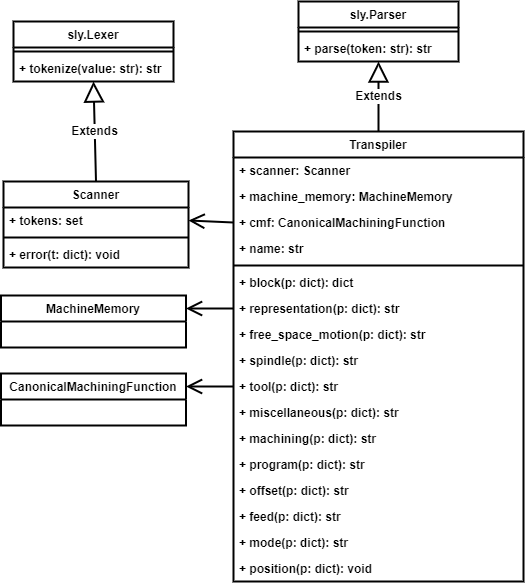
\includegraphics[width=4.5cm]{ncparser-class-transpiler.png}
%     \end{subfigure}
%     %\qquad
%     \begin{subfigure}[b]{0.8\textwidth}
%       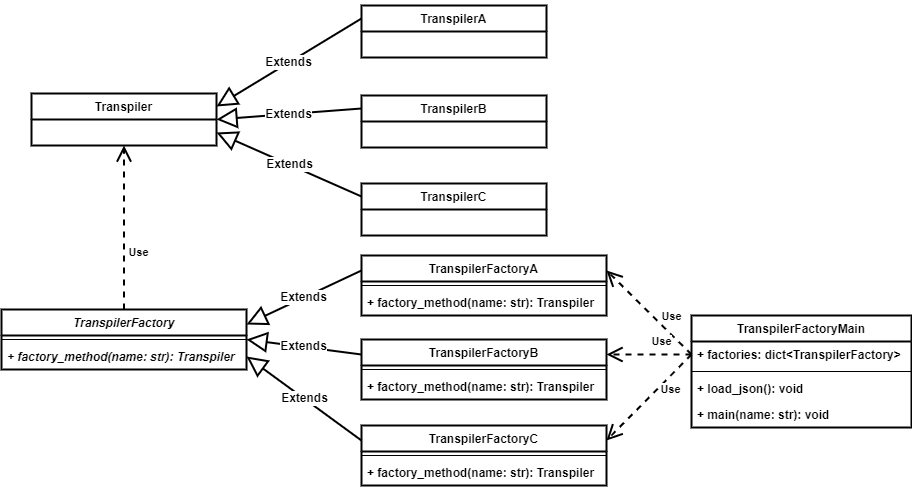
\includegraphics[width=6.5cm]{ncparser-class-transpiler-factory.png}        
%     \end{subfigure}
%     %\caption{Diagrama de Classes}
% \end{figure}


% \subsection{Resultados esperados}
% \begin{frame}{Resultados esperados}
%   \begin{itemize}
%     \item Implementar uma camada abstrata para o registro temporal dos eventos decorrentes do 
%     processamento do programa de controle num\'erico.
%     \item Implementar um aplicativo para o processamento de dialetos de programas de controle 
%     num\'erico industriais.
%     \item Publicar artigo em anais de congressos cient\'ificos.
%     \item Publicar artigo em revista cient\'ifica.
%     \item Fazer o registro do software desenvolvido.
%   \end{itemize}
% \end{frame}




% \subsection{Resultados já alcançados}
% \begin{frame}{Resultados já alcançados}
%   \begin{itemize}
%     \item {
%       A metodologia para a transpila\c c\~ao do arquivo CN para as Fun\c c\~oes Can\^onicas de Usinagem 
%       foi publicada em um artigo cient\'ifico para o 26\textordmasculine Congresso Internacional de 
%       Engenharia Mec\^anica (COBEM 2021), realizado entre os dias 22 e 26 de Novembro de 2021.
%       O t\'itulo do artigo publicado foi \emph{Transpilation from NC Files to Canonical 
%       Machining Functions}.
%     }
%     \item {
%       Outro resultado j\'a alcan\c cado, no contexto do projeto proposto, foi a contribui\c c\~ao no 
%       trabalho do mestrando Vin\'icius Otto Mehl, com o t\'itulo 
%       \emph{Avalia\c c\~ao em tempo real da efetividade global de uma linha de usinagem do tipo transfer}.
%     }
%   \end{itemize}
% \end{frame}


% \subsection{Estudo de Caso}

% \begin{frame}{Objetivos Específicos}
%   \begin{itemize}
%     \item {
%       Interpretar programas de controle num\'erico, escritos em um determinado dialeto do 
%       padr\~ao RS-274D, e convert\^e-los para um outro nível de abstração:
%       \begin{itemize}
%         \item Formato Padronizado;
%         \item Capaz de descrever cada movimento feito durante a usinagem.
%       \end{itemize}
%     }
%     \item {
%       Modelar os \emph{features} de usinagem a partir de um projeto orientado a objetos.
%     }
%     \item {
%       Processar os arquivos de Fun\c c\~oes Can\^onicas de Usinagem e extrair os dados 
%       temporais.
%     }
%   \end{itemize}
% \end{frame}


% Placing a * after \section means it will not show in the
% outline or table of contents.

% \section*{Summary}

% \begin{frame}{Summary}
%   \begin{itemize}
%   \item
%     The \alert{first main message} of your talk in one or two lines.
%   \item
%     The \alert{second main message} of your talk in one or two lines.
%   \item
%     Perhaps a \alert{third message}, but not more than that.
%   \end{itemize}
  
%   \begin{itemize}
%   \item
%     Outlook
%     \begin{itemize}
%     \item
%       Something you haven't solved.
%     \item
%       Something else you haven't solved.
%     \end{itemize}
%   \end{itemize}
% \end{frame}


% All of the following is optional and typically not needed. 
  % \appendix
  % \section<presentation>*{\appendixname}
  % \subsection<presentation>*{For Further Reading}

  % \begin{frame}[allowframebreaks]
  %   \frametitle<presentation>{For Further Reading}
      
  %   \begin{thebibliography}{10}
      
  %   \beamertemplatebookbibitems
  %   % Start with overview books.

  %   \bibitem{Author1990}
  %     A.~Author.
  %     \newblock {\em Handbook of Everything}.
  %     \newblock Some Press, 1990.
  
      
  %   \beamertemplatearticlebibitems
  %   % Followed by interesting articles. Keep the list short. 

  %   \bibitem{Someone2000}
  %     S.~Someone.
  %     \newblock On this and that.
  %     \newblock {\em Journal of This and That}, 2(1):50--100,
  %     2000.
  %   \end{thebibliography}
  % \end{frame}

  % }
